\documentclass[nobib]{tufte-handout}

\title{Föreläsning 6: Fortsättning på genererande funktioner $\cdot$ 1MA020}

\author[Vilhelm Agdur]{Vilhelm Agdur\thanks{\href{mailto:vilhelm.agdur@math.uu.se}{\nolinkurl{vilhelm.agdur@math.uu.se}}}}

\date{7 februari 2023}


%\geometry{showframe} % display margins for debugging page layout

\usepackage{graphicx} % allow embedded images
  \setkeys{Gin}{width=\linewidth,totalheight=\textheight,keepaspectratio}
  \graphicspath{{graphics/}} % set of paths to search for images
\usepackage{amsmath}  % extended mathematics
\usepackage{booktabs} % book-quality tables
\usepackage{units}    % non-stacked fractions and better unit spacing
\usepackage{multicol} % multiple column layout facilities
\usepackage{lipsum}   % filler text
\usepackage{fancyvrb} % extended verbatim environments
  \fvset{fontsize=\normalsize}% default font size for fancy-verbatim environments

\usepackage{color,soul} % Highlights for text


\include{mathcommands.extratex}

\begin{document}

\definecolor{darkgreen}{rgb}{0.0627, 0.4588, 0.1451}

\maketitle% this prints the handout title, author, and date

\begin{abstract}
\noindent
Vi fortsätter förra föreläsningens diskussion om genererande funktioner, och använder dem för att räkna lösningar till ekvationer. Sedan introducerar vi exponentiella genererande funktioner, och använder dessa för att lösa några problem.
\end{abstract}

\section{Antal lösningar till en ekvation, med begränsningar}

I slutet på förra föreläsningen studerade vi antalet lösningar till ekvationen
$$x_1 + x_2 + x_3 + x_4 + x_5 = k$$
om vi kräver att alla $x_i$ är ickenegativa heltal. Det var ett första exempel på en mer generell kategori av problem med att räkna lösningar på ekvationer. Låt oss börja med ett lite mer invecklat problem:

\begin{example}
    Hur många lösningar finns det till
    $$x_1 + x_2 + x_3 + x_4 = k$$
    om vi kräver att alla $x_i$ är ickenegativa heltal, men också kräver att $x_2$ är jämnt, att $x_3 \leq 10$, och $x_4$ är udda?

    Låt, för varje $k$, $a_k$ vara antalet sådana lösningar.
    Låt sedan $a_k^1$ vara antalet lösningar till $x_1 = k$ i ickenegativa heltal $x_1$,
    $a_k^2$ vara antalet lösningar till $x_2=k$ i ickenegativa jämna heltal,
    $a_k^3$ vara antalet lösningar till $x_3=k$ i heltal mellan $0$ och $10$,
    och $a_k^4$ vara antalet lösningar till $x_4 = k$ i udda heltal.

    Precis som i förra exemplet studerar vi nu faltningen av dessa fyra följder, och ser att
    $$(a^1 * a^2 * a^3 * a^4)_k = \sum_{\substack{k_1, k_2, k_3, k_4\geq 0\\k_1 + k_2 + k_3 + k_4 = k}} a_{k_1}^1a_{k_2}^2a_{k_3}^3a_{k_4}^4 = a_k$$
    eftersom $a_{k_1}^1a_{k_2}^2a_{k_3}^3a_{k_4}^4$ är en produkt av ettor och nollor -- att $k_1 + k_2 + k_3 + k_4 = k$ garanteras av definitionen av faltning, och sedan är varje term i produkten ett om värdet på $k_i$ är tillåtet av våra begränsningar, och noll annars. Så produkten är ett om summan är korrekt och varje enskild begränsning är uppfylld.

    Så precis som i förra exemplet kan vi få fram genererande funktionen för $a_k$, följden vi faktiskt är intresserade av, genom att plocka fram den genererande funktionen för de enklare följderna.

    Vad genererande funktionen för $a^1$ är vet vi sedan innan -- den är bara en följd av ettor, så dess genererande funktion blir $\frac{1}{1-x}$. Likaledes vet vi sedan innan att följden av $n$ stycken ettor och sedan nollor har genererande funktion $\frac{1 - x^{n+1}}{1-x}$, så genererande funktionen för $a^3$ blir $\frac{1 - x^{11}}{1-x}$.

    Däremot för $a^2$ behöver vi räkna ut något nytt, nämligen den genererande funktionen för följden $1,0,1,0,1,\ldots$, indikatorfunktionen av de jämna talen. Så vi får skriva att
    \begin{align*}
        F_{a^2}(x) &= \sum_{k=0}^{\infty} a^2_k x^k\\
        &= \sum_{\substack{k \geq 0\\k \in 2\Z}} x^k\\
        &= \sum_{i=0}^{\infty} x^{2i}\\
        &= \sum_{i=0}^{\infty} (x^2)^i
    \end{align*}
    och sista raden här kan vi känna igen som genererande funktionen av följden $(1,1,1,1,\ldots)$, \emph{utvärderad i} $x^2$. Så detta är lika med $\frac{1}{1-x^2}$.

    Så vad som återstår är alltså $a^4$, indikatorfunktionen för de udda talen. För att få fram dess genererande funktion kan vi använda vad vi just gjorde för de jämna talen:
    \begin{align*}
        F_{a^4}(x) &= \sum_{k=0}^{\infty} a_k x^k\\
        &= \sum_{\substack{k \geq 1\\k\text{ udda}}} x^k\\
        &= x\sum_{\substack{k \geq 1\\k\text{ udda}}} x^{k-1}\\
        &= x\sum_{\substack{k \geq 0\\k \in 2\Z}} x^k\\
        &= \frac{x}{1 - x^2}.
    \end{align*}

    Så, om vi använder att genererande produkten av en faltning är produkten av de genererande funktionerna, ser vi att
    \begin{align*}
        F_a(x) &= \left(\frac{1}{1-x}\right)\left(\frac{1-x^{11}}{1-x}\right)\left(\frac{1}{1-x^2}\right)\left(\frac{x}{1-x^2}\right)\\
        &= \frac{x(1 - x^{11})}{(1-x)^2(1-x^2)^2}
    \end{align*}
    och ber vi vårt favorit-CAS\sidenote[][]{\emph{Computer Algebra System}, alltså till exempel \emph{WolframAlpha} eller något av dess öppna alternativ, såsom \emph{Sage}.} att Taylorutvidga detta uttryck så får vi att
    $$F_a(x) = x + 2x^2 + 5x^3 + 8x^4 + 14x^5 + 20x^6 + 30x^7 + 40x^8 + \ldots$$
    så att följden av antalet lösningar är
    $$0,1,2,5,8,14,20,30,40,55,70,91,111,138,163,\ldots.$$
\end{example}

\begin{example}
  Vi vill räkna antalet lösningar $a_k$ till ekvationen
  $$2x_1 + x_2 + x_3 = k$$
  där alla $x_i$ är heltal, $x_2$ är en multipel av $6$, och talet $x_3$ kan vara antingen rött eller blått.\sidenote[][]{Vi ser alltså, för $k = 6$, alla dessa som godtagbara distinkta lösningar:
  $$x_1 = 1, x_2 = 0, x_3 = \textcolor{blue}{4}, \qquad x_1 = 1, x_2 = 0, x_3 = \textcolor{red}{4},$$
  $$x_1 = 2, x_2 = 0, x_3 = \textcolor{blue}{2}, \qquad x_1 = 0, x_2 = 6, x_3 = \textcolor{red}{0}.$$}

  Vi börjar med att göra variabelbytet $y_1 = 2x_1$, och vill alltså nu ha lösningar till $y_1 + x_2 + x_3 = k$, med begränsningen att $y_1$ är jämnt. Det här förändrar så klart inte antalet lösningar, bara gör det lättare för oss att tillämpa vår metod.

  Vi tillämpar samma metod som i förra exemplet, och låter $a^1_k$ vara antalet lösningar till $y_1 = k$ med $y_1$ jämnt, $a^2_k$ vara antalet lösningar till $x_2 = k$ med $x_2$ delbart med $6$, och $a^3_k$ vara antalet lösningar till $x_3 = k$ med $x_3$ färgat antingen rött eller blått. Faltningen blir då 
  $$(a^1 * a^2 * a^3)_k = \sum_{\substack{k_1, k_2, k_3 \geq 0\\k_1+k_2+k_3 = k}} a^1_{k_1}a^2_{k_2}a^3_{k_3} = a_k.$$

  Vi fortsätter precis som innan med att räkna ut den genererande funktionen för varje av våra följder. För $a^1$ vet vi redan vad genererande funktionen för indikatorfunktionen av de jämna talen är, nämligen $\frac{1}{1-x^2}$. 
  
  För $a^2$ kan vi använda samma metod som vi använde för de jämna talen för att se att
  \begin{align*}
    F_{a^2}(x) &= \sum_{k=0}^{\infty} a^2_k x^k = \sum_{\substack{k \geq 0\\k \in 6\Z}} x^k\\
    &= \sum_{i=0}^{\infty} x^{6i} = \sum_{i=0}^{\infty} (x^6)^i
  \end{align*}
  så att $F_{a^2}(x) = \frac{1}{1-x^6}$.

  För $a^3$ så blir denna helt enkelt en följd av bara tvåor, eftersom vi har två val för färg för varje tal, och kan välja vilket tal som helst. Så vi ser att
  $$F_{a^3}(x) = \sum_{k=0}^{\infty} 2x^k = 2\frac{1}{1-x}.$$

  Sammantaget har vi alltså att
  $$F_a(x) = \left(\frac{1}{1-x^2}\right)\left(\frac{1}{1-x^6}\right)\left(\frac{2}{1-x}\right) = \frac{2}{(1-x)(1-x^2)(1-x^6)}$$
  vilket vi kan Taylorutvidga i vårt favoritprogram och få att\sidenote[][]{Vi ser ju ett tydligt mönster här av att $a_{2k} = a_{2k+1}$. Kan du förklara varför detta måste vara fallet, baserat på våra begränsningar av variablerna?}
  \begin{align*}
    F_a(x) &= 2 + 2 x + 4 x^2 + 4 x^3 + 6 x^4 + 6 x^5 + 10 x^6 + 10 x^7\\
    & + 14 x^8 + 14 x^9 + 18 x^{10} + 18 x^{11} + 24 x^{12} + 24 x^{13}\\
    & + 30 x^{14} + 30 x^{15} + 36 x^{16} + 36 x^{17} + 44 x^{18} + \ldots.
  \end{align*}
\end{example}

\section{Att omvandla ett problem till en rekursion}

Vårt nästa exempel handlar inte om att räkna lösningar till en ekvation, utan om att översätta ett problem till en rekursion. Vi tar detta exemplet nu delvis eftersom vi kommer vilja ha en rekursion att lösa i ett senare exempel.

\begin{example}
  Antag att vi har ett schackbräde med $2\times n$ rutor, och vi vill täcka det med brickor av formen $2\times 1$ eller $1\times 2$. Hur många sätt kan vi göra detta på?

  \begin{marginfigure}
    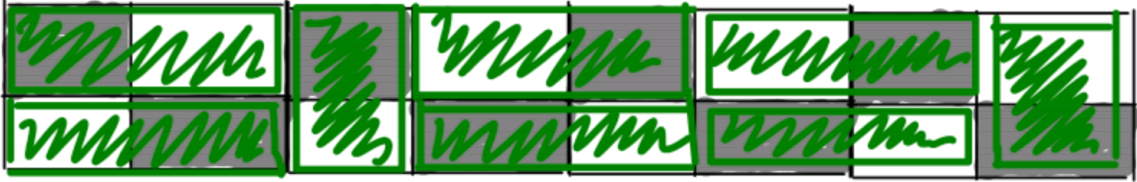
\includegraphics{graphics/checkerboard_tiling.png}
    \caption{Ett sätt att göra detta då $n=8$. Figur tagen ur förra årets anteckningar.}
  \end{marginfigure}

  Låt $t_n$ vara antalet sätt vi kan täcka vårt schackbräde. Vi vill hitta en rekursion för detta antal. Vi ser enkelt att det finns ett enda sätt att göra det för $n=1$ -- bara en bricka får plats -- så $t_1 = 1$. För $n=2$ finns det två sätt, antingen lägger vi dem horisontellt eller vertikalt, så $t_2 = 2$.

  \begin{marginfigure}
    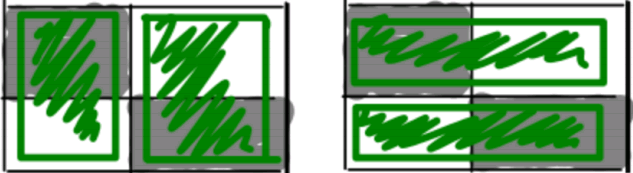
\includegraphics{graphics/checkerboard_tiling_n_2.png}
    \caption{De två sätten att göra det på då $n=2$. Figur från förra årets föreläsningsanteckningar.}
  \end{marginfigure}

  Om vi vill skapa oss en täckning av en $2\times n$-bräda, för något $n > 2$, kan vi göra på två sätt:
  \begin{itemize}
    \item Vi börjar med en täckning av en $2\times(n-1)$-bräda, och lägger till en till bricka vertikalt.
    \item Vi börjar med en täckning av en $2\times(n-2)$-bräda, och lägger till två till brickor horisontellt.
  \end{itemize}

  Att varje täckning av en $2\times n$-bräda kan skapas på detta vis är enkelt att se -- antingen är den sista kolumnen täckt av en vertikal bricka, i vilket fall vi skapade täckningen på första viset, eller så är den täckt av två horisontella brickor, i vilket fall vi skapade den på det andra sättet.

  Alltså har vi funnit följande rekursion för antalet täckningar
  $$t_0 = 0, t_1 = 1, t_2 = 2, \quad t_n = t_{n-1} + t_{n-2} \, \forall n > 2$$
  som ju är extremt lik den vi har för Fibonaccitalen, så vi kan finna en genererande funktion och sluten form på precis samma vis som i det fallet.
\end{example}

\section{Exponentiella genererande funktioner}

Ibland får vi problem med att hitta enkla uttryck för våra genererande funktioner, eftersom vår följd växer för snabbt. Hittills har vi bara studerat följder som växer långsamt nog, men om vi till exempel hade velat studera följden $0!, 1!, 2!,\ldots$ hade dess vanliga genererande funktion varit 
$$\sum_{k=0}^{\infty} k!x^k$$
för vilken det inte finns något enkelt uttryck.\sidenote[][]{Om vi sätter på oss våra analytiker-glasögon kan vi dessutom se att detta uttryck inte konvergerar för något $x > 0$, så vad hade vi ens kunna ha för uttryck för en funktion som är oändlig överallt?}

Ett annat exempel på detta är om vi räknar permutationer -- dessa kommer vara ungefär $k!$ stycken, i de flesta av våra exempel. Så vi hade haft samma problem. Det finns en anledning att vi hittills bara studerat binomialkoefficienter, som ju är betydligt mindre.

Så, låt oss definiera en variant på genererande funktioner som kan hantera dessa snabbväxande följder.

\begin{definition}
  Om $\{a_k\}_{k=0}^\infty$ är någon följd ges dess \emph{exponentiella genererande funktion} av\sidenote[][]{Om vi behöver förtydliga skillnaden kallar vi de icke-exponentiella genererande funktionerna vi studerade innan för \emph{ordinära} genererande funktioner.}
  $$EG_a(x) = \sum_{k=0}^{\infty} a_k \frac{x^k}{k!}.$$
\end{definition}

Så allt vi faktiskt har gjort är att skala ner vår följd så att den inte växer så kraftigt. Som tur är fungerar detta enkla trick väldigt väl -- låt oss räkna några exempel för att se hur.

\begin{example}
  Den exponentiella genererande funktionen för följden $(1,1,1,1,\ldots)$ ges av
  $$\sum_{k=0}^{\infty} \frac{x^k}{k!} = e^x.$$
\end{example}

\begin{example}
  Den exponentiella genererande funktionen för följden $(0!, 1!, 2!, 3!, \ldots)$ ges av
  $$\sum_{k=0}^{\infty} k!\frac{x^k}{k!} = \sum_{k=0}^{\infty} x^k = \frac{1}{1-x}.$$
\end{example}

\begin{example}
  Fixera något heltal $n$, och låt $a_k$ vara antalet permutationer av längd $k$ ur ett alfabete med $n$ bokstäver, så att $a_k = \frac{n!}{(n-k)!}$. Då ges den exponentiella genererande funktionen för $a$ av
  \begin{align*}
    EG_a(x) &= \sum_{k=0}^{\infty} \frac{n!}{(n-k)!}\frac{x^k}{k!}\\
    &= \sum_{k=0}^{\infty} \frac{n!}{k!(n-k)!}x^k\\
    &= \sum_{k=0}^{\infty} \binom{n}{k} x^k = (1 + x)^n
  \end{align*}
  där vi i sista ledet kände igen en \emph{ordinär} genererande funktion för binomialkoefficienterna.
\end{example}

\begin{example}
  Låt oss återvända till exemplet med schackbrädena. Vi hade en följd som gavs av rekursionen\sidenote[][]{Notera att vi har ändrat om i rekursionen så att vi har plustecken i index istället för minus -- det är fortfarande precis samma rekursion, men vi får finare uttryck senare.}
  $$t_0 = 0, t_1 = 1, t_2 = 2, \quad t_{k+2} = t_{k+1} + t_{k} \, \forall k \geq 1.$$

  Vad är den exponentiella genererande funktionen för denna följden? Analogt med det ordinära fallet tar vi vår rekursion, multiplicerar den med $\frac{x^k}{k!}$, och summerar över alla $k \geq 1$, för att få att
  $$\sum_{k=1}^{\infty} t_{k+2} \frac{x^k}{k!} = \sum_{k=1}^{\infty} t_{k+1}\frac{x^k}{k!} + \sum_{k=1}^{\infty} t_{k}\frac{x^k}{k!}.$$

  Nu kan vi komma ihåg att
  $$\frac{\intd}{\dx} \frac{x^k}{k!} = \frac{x^{k-1}}{(k-1)!}$$
  så att
  $$t_{k+1}\frac{x^k}{k!} = t_{k+1}\left(\frac{\intd}{\dx} \frac{x^{k+1}}{(k+1)!}\right)$$
  och
  $$t_{k+2}\frac{x^k}{k!} = t_{k+2}\left(\frac{\intd^2}{\intd x^2} \frac{x^{k+2}}{(k+2)!}\right).$$

  Om vi använder dessa likheter i vad vi hade innan, och bryter ut derivatorna ur summorna, får vi alltså att
  $$\frac{\intd^2}{\intd x^2}\left(\sum_{k=1}^{\infty} t_{k+2} \frac{x^{k+2}}{(k+2)!}\right) = \frac{\intd}{\dx}\left(\sum_{k=1}^{\infty} t_{k+1}\frac{x^{k+1}}{(k+1)!}\right) + \left(\sum_{k=1}^{\infty} t_{k}\frac{x^k}{k!}\right).$$

  Precis som i vårt exempel med Fibonaccitalen ser vi nu att vi nästan har de exponentiella genererande funktionerna, förutom att det saknas några av de första termerna i summorna. Så om vi justerar för detta får vi att
  \begin{align*}
    \frac{\intd^2}{\intd x^2}\left(EG_t(x) - t_0\frac{x^0}{0!} - t_1\frac{x^1}{1!} - t_2\frac{x^2}{2!}\right) &=\\
    = \frac{\intd}{\dx}\left(EG_t(x) - t_0\frac{x^0}{0!} - t_1\frac{x^1}{1!}\right)& + \left(EG_t(x) - t_0\frac{x^0}{0!}\right)
  \end{align*}
  så om vi substituerar in $t_0 = 0, t_1 = 1, t_2 = 2$ och flyttar in derivatorna i parenteserna så får vi att
  $$EG_t''(x) - 2 = EG_t'(x) - 1 + EG_t(x)$$
  vilket ju är en helt vanlig andra gradens linjär ordinär differentialekvation med konstanta koefficienter. Randvillkoren för den ges av $EG_t(0) = t_0$ och $EG_t'(0) = t_1$.\sidenote[][]{Detta kommer ju alltid gälla för alla exponentiella genererande funktioner, av hur de är definierade.}
  
  Så vi kan antingen lösa den för hand eller med hjälp av vårt favorit-CAS, och finna lösningen
  $$\frac{1}{10} \left(\sqrt{5} e^{\left(\frac{\sqrt{5}}{2}+\frac{1}{2}\right) x}-\sqrt{5} e^{\left(\frac{1}{2}-\frac{\sqrt{5}}{2}\right) x}+5 e^{\left(\frac{\sqrt{5}}{2}+\frac{1}{2}\right) x}+5 e^{\left(\frac{1}{2}-\frac{\sqrt{5}}{2}\right) x}-10\right)$$
  vilket vår CAS\sidenote[][]{Eller vi, för hand, om vi inte är lata. Den enda funktionen som är involverad är ju $e^x$, så det är inget svårt att expandera, bara många termer att hålla ordning på.} låter oss se kan Taylorutvidgas till
  $$\sum_{n=1}^{\infty} \frac{\left(5 - \sqrt{5}\right) \left(\frac{1 - \sqrt{5}}{2}\right)^n + \left(5 + \sqrt{5}\right) \left(\frac{1 + \sqrt{5}}{2}\right)^n}{10} \frac{x^n}{n!}$$
  vilket alltså ger oss en direkt formel för varje term i följden, i samma still som för Fibonaccitalen.
\end{example}

Vad vi sett i detta exemplet är alltså att vi, när vi har en felmatchning mellan index i vår följd och index i $\frac{x^k}{k!}$, plockar på oss derivator -- till skillnad från i fallet med ordinära genererande funktioner, då detta gav oss faktorer av $x$.

Vi har också sett att de exponentiella genererande funktioner vi hittar för linjära rekursioner kommer ha en bunt olika $e^{Cx}$ för konstanter $C$,\sidenote[][]{Precis som vi såg för följden $(1,1,1,\ldots)$, där $C = 1$ -- detta beror, i alla fall andligen, på att våra följder som ges av linjära rekursioner också kommer växa ungefär så långsamt, så vi får samma sorts funktion.} vilket är mycket enklare att Taylorutvidga. Så om man vill lösa linjära rekursioner i praktiken är exponentiella genererande funktioner ofta ett bättre val än ordinära.

\section{Binomial-faltningar och EGFer}

Vi har lärt oss att motsvarigheten till en faltning på den kombinatoriska sidan är en produkt av genererande funktioner. Vad händer om vi i stället tar \emph{exponentiella} genererande funktioner? Situationen blir lite mer komplicerad.

\begin{definition}
  Antag att $\{a_k\}_{k=0}^\infty$ och $\{b_k\}_{k=0}^\infty$ är två följder. Då ges deras \emph{binomial-faltning} $a \ostar b$ av
  $$(a \ostar b)_k = \sum_{i=0}^{k} \binom{k}{i} a_i b_{k-i}.$$
\end{definition}

\begin{lemma}
  Antag att $\{a_k\}_{k=0}^\infty$ och $\{b_k\}_{k=0}^\infty$ är två följder, vars exponentiella genererande funktioner är $EG_a(x)$ och $EG_b(x)$. Då ges den genererande funktionen för binomial-faltningen $a \ostar b$ av
  $$EG_{a \ostar b}(x) = EG_a(x)EG_b(x)$$

  \begin{proof}
    Lägg märke till att $EG_a$ inte bara är den exponentiella genererande funktionen för $a$, utan också är den ordinära genererande funktionen för $A_k = \frac{a_k}{k!}$, och likaledes för $b$. Alltså måste, enligt vad vi redan vet om ordinära genererande funktioner,
    $$EG_a(x)EG_b(x) = G_{A}(x)G_{B}(x) = G_{A * B}(x).$$

    Så vad vi studerar är den vanliga faltningen av $A$ med $B$ -- vi ser att denna är
    \begin{align*}
      \left(A * B\right)_k &= \sum_{i=0}^{k} A_{i}B_{k-i}\\
      &= \sum_{i=0}^{k} \frac{a_i}{i!}\frac{b_{k-i}}{(k-i)!}\\
      &= \sum_{i=0}^{k} \frac{k!}{i!(k-i)!}\frac{a_i b_{k-i}}{k!}\\
      &= \sum_{i=0}^{k} \binom{k}{i}a_i b_{k-i}\frac{1}{k!} = (a \ostar b)_k \frac{1}{k!}
    \end{align*}
    så alltså måste vi ha
    \begin{align*}
      G_{A * B}(x) &= \sum_{k=0}^\infty (A*B)_k x^k\\
      &= \sum_{k=0}^{\infty}(a\ostar b)_k \frac{x^k}{k!}\\
      &= EG_{a \ostar b}(x)
    \end{align*}
    och vårt lemma är bevisat.
  \end{proof}
\end{lemma}

På ett fullkomligt analogt sätt, användandes resultatet för ordinära genererande funktioner, fast med fler index, kan vi bevisa följande resultat:
\begin{lemma}
  Antag att $\{a^1_k\}_{k=0}^\infty, \{a^2_k\}_{k=0}^\infty, \ldots, \{a^d_k\}_{k=0}^\infty$ är följder. Då gäller det att\sidenote[][]{Kom ihåg att notationen $\binom{k}{k_1, k_2, \ldots, k_d}$ betecknar en \emph{multinomialkoefficient}.}
  $$(a^1 \ostar a^2 \ostar \ldots \ostar a^d)_k = \sum_{\substack{k_1, k_2, \ldots, k_d\\k_1 + k_2 + \ldots + k_d = k}} \left(\binom{k}{k_1, k_2, \ldots, k_d} \prod_{j=1}^{d} a^j_{k_j}\right)$$
  och
  $$EG_{a^1 \ostar a^2 \ostar \ldots \ostar a^d}(x) = \prod_{j=1}^{d} EG_{a^j}(x).$$
\end{lemma}

Som vårt sista exempel för denna föreläsning tar vi motsvarigheten för exponentiella genererande funktioner till våra problem med antal lösningar på en ekvation.

\begin{example}
  Hur många strängar ur alfabetet $\{a, b, c, d\}$ finns det av längd $k$, med åtminstone ett $b$, högst tre $c$, och ett jämnt antal $d$?

  Precis som i fallet med att räkna lösningar till ekvationer låter vi $l_k$ vara antalet sådana strängar, och låter sedan
  \begin{itemize}
    \item $a_k$ vara antalet strängar ur alfabetet $\{a\}$ av längd $k$,
    \item $b_k$ vara antalet strängar ur alfabetet $\{b\}$ av längd $k$ med åtminstone ett $b$,
    \item $c_k$ vara antalet strängar ur alfabetet $\{c\}$ av längd $k$ med högst tre $c$, och
    \item $d_k$ vara antalet strängar ur alfabetet $\{d\}$ av längd $k$ med ett jämnt antal $d$.
  \end{itemize}

  Om vi nu betraktar binomialfaltningen av dessa fyra följder ser vi att
  $$(a \ostar b \ostar c \ostar d)_k = \sum_{\substack{k_1, k_2, k_3, k_4\\k_1 + k_2 + k_3 + k_4 = k}} \binom{k}{k_1, k_2, k_3, k_4} a_{k_1}b_{k_2}c_{k_3}d_{k_4} = l_k$$
  eftersom vad vi räknar med multinomialkoefficienten $\binom{k}{k_1, k_2, k_3, k_4}$ är precis antalet strängar av längd $k$ med $k_1$ stycken $a$, $k_2$ stycken $b$, och så vidare.

  Vad som återstår är alltså att finna de exponentiella genererande funktionerna för våra fyra följder.
  \begin{itemize}
    \item Följden $a$ är helt enkelt $(1,1,1,\ldots)$, så dess exponentiella genererande funktion har vi redan sett är $e^x$.
    \item Följden $b$ är $(0,1,1,\ldots)$, så vi kan räkna att 
    $$EG_b(x) = \sum_{k=1}^{\infty} \frac{x^k}{k!} = \sum_{k=0}^{\infty} \frac{x^k}{k!} - 1 = e^x - 1.$$
    \item Följden $c$ är $(1,1,1,1,0,0,\ldots)$, så 
    $$EG_c(x) = 1 + x + \frac{x^2}{2} + \frac{x^3}{6}.$$
    \item För följden $d$ får vi använda oss av ett litet trick, och skriva att 
    \begin{align*}
      EG_d(x) &= \sum_{k \in 2\Z^{\geq 0}} \frac{x^k}{k!}\\
      &= \frac{1}{2}\left(\sum_{k=0}^{\infty} \frac{x^k}{k!} - \sum_{k=0}^{\infty} \frac{(-x)^k}{k!}\right)\\
      &= \frac{e^x - e^{-x}}{2}.
    \end{align*}
  \end{itemize}

  Multiplicerar vi ihop dessa får vi att 
  $$EG_l(x) = e^x\left(e^x - 1\right)\left(1 + x + \frac{x^2}{2} + \frac{x^3}{3}\right)\left(\frac{e^x - e^{-x}}{2}\right).$$
  
  Om vi vill ha en explicit formel är ett bra nog CAS\sidenote[][]{Mathematica kan det, men inte WolframAlpha.} kapabelt att ge en explicit formel för den $n$te termen i serieexpansionen av detta, men den är inte vacker.
\end{example}

\section{Övningar}

\begin{xca}
  Hur många heltalslösningar till ekvationen
  $$x_1 + x_2 + x_3 = 578$$
  finns det,\sidenote[][-2cm]{Om ni väl har hittat genererande funktionen för antalet lösningar när vi ersatt $578$ med $k$, så kan ni enkelt få fram svaret med följande kod till \emph{WolframAlpha}:
  $$\mathtt{SeriesCoefficient}[f, \{x,0,578\}]$$
  där $f$ då är genererande funktionen ni funnit. Att ange den genererande funktionen och säga att ni sedan plockade fram rätt koefficient ur den med hjälp av ett CAS är den förväntade metoden här.} om vi kräver att
  \begin{itemize}
    \item $x_1 \geq -7$,\sidenote[][]{Ledtråd: Gör ett variabelbyte till $y_1$ för att få den vanliga begränsningen att $y_1 \geq 0$.}
    \item $x_2 \geq 0$ är ett jämnt tal,
    \item och $x_3 \geq 0$ kan vara vilket tal som helst, men om det är jämnt kan det vara rött eller blått, och om det är udda kan det vara gult, grönt, eller lila. 
  \end{itemize}
\end{xca}

\begin{xca}
  Antag att vi vet att följden $\{a_k\}_{k=0}^\infty$ har exponentiell generande funktion $F$. Finn ett enkelt uttryck för den exponentiella genererande funktionen för följden $b_k = k a_k$, i termer av $F$.
\end{xca}

\begin{xca}
  I denna övning använder vi ett lite mer abstrakt språk. Låt $\mathfrak{F}$ vara mängden av alla följder, och $\mathfrak{G}$ vara mängden av alla genererande funktioner. Då kan vi alltså låta $G: \mathfrak{F} \to \mathfrak{G}$ vara funktionen som skickar en följd till dess ordinära genererande funktion, och $EG: \mathfrak{F} \to \mathfrak{G}$ funktionen som skickar en följd till dess exponentiella genererande funktion.

  Vi kan också definiera operatorn (funktionen) $A: \mathfrak{F} \to \mathfrak{F}$ som att $(Aa)_k = a_{k+1}$. Vi förskjuter alltså index ett steg, och slänger bort första termen i vår följd.\sidenote[][]{Så till exempel har vi att $A(1,0,1,0,1,0,\ldots) = (0,1,0,1,0,1,\ldots)$.} Likaledes kan vi definiera operatorn $D: \mathfrak{G} \to \mathfrak{G}$ som funktionen som skickar en genererande funktion på dess derivata.\sidenote[][]{Vi har ju egentligen inte \emph{definierat} vad vi menar med derivatan av en genererande funktion, utan bara låtsats att vi får behandla dem som vilken funktion som helst, och ignorerat alla konvergensfrågor och allt krångel om att summorna har oändligt med termer. Vi fortsätter att göra så.}

  Slutligen kan vi, för varje heltal $n$, definiera operatorn $T_n: \mathfrak{F} \to \R$ som att $Ta = a_n$. Den plockar alltså helt enkelt ut den $n$te termen i följden.

  Låt oss nu plocka ner all denna abstraktionen på en lite mer konkret nivå. Övertyga er själva, genom att skriva ut konkret vad påståendena betyder, om att vi redan visat i föreläsningarna att
  \begin{itemize}
    \item $G(A(a)) = \frac{1}{x}\left(G(a) - T_0(a)\right)$ och
    \item $EG(A(a)) = D(EG(a))$. Vill man vara oerhört förfinad och abstrakt kan man formulera detta som att följande diagram kommuterar:
    
    \begin{center}
      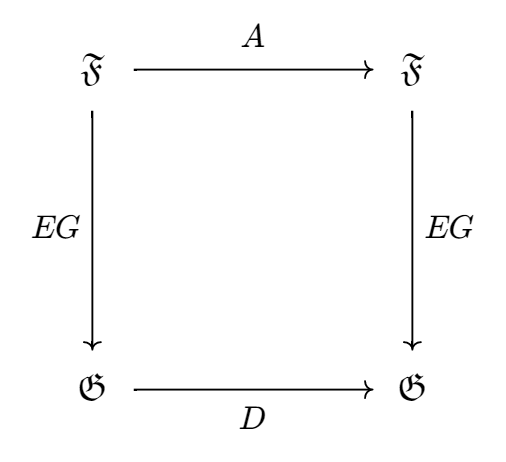
\includegraphics[width=0.4\textwidth]{graphics/abstract_exercise_comm_diag.png}
    \end{center}
  \end{itemize}
\end{xca}

\begin{xca}
  Låt oss nu se varför detta abstrakta språk faktiskt är användbart ibland.\sidenote[][]{I det här fallet ger det oss ett mycket koncisare sätt att uttrycka räkningen för att hitta genererande funktionen för indikatorföljden för talen delbara med tre. Dessutom blir det tydligt hur man hade gjort om vi hade sju istället för tre.
  
  Kanske att man till och med kan göra räkningen för godtyckliga $n\Z$, men det kräver nog mer differentialekvationsteori än jag kan, eller kan förvänta mig att ni skall kunna. (Jag försökte i ungefär en minut med Laplacetransformer, men det blev svårt och kändes invecklat.)} Låt $a = (1,0,0,1,0,0,1,\ldots)$, och låt $\overrightarrow{1} = (1,1,1,\ldots)$.

  Visa att
  $$a = \overrightarrow{1} - Aa - AAa,$$
  använd vad vi just gjorde i förra övningen för att omvandla detta till en differentialekvation för $EG(a)$, och lös differentialekvationen\sidenote[][]{Det här steget vill jag inte ha några räkningar på -- bara ange vad lösningen blir. Ni får använda vilket verktyg ni vill för att faktiskt lösa den.} för att få fram ett uttryck för exponentiella genererande funktionen för $a$.
\end{xca}

\begin{xca}
  Låt $\ell_k$ vara antalet strängar ur alfabetet $\{a,b,c\}$ av längd $k$, sådana att
  \begin{itemize}
    \item det omedelbart efter varje $a$ följer ett $b$,\sidenote[][]{Ledtråd: För att hantera denna begränsning behöver vi göra ett ``variabelbyte''. Vad kan det tänkas betyda i denna kontext?}
    \item det finns ett jämnt antal $c$,
    \item antalet $a$ är delbart med tre,
    \item och varje $b$ föregås av ett $a$?
  \end{itemize}

  Finn genererande funktionen för följden $\ell_k$.
\end{xca}

\begin{xca}
  För varje $n$ ges det $n$te \emph{Bell-talet} av
  $$B_n = \sum_{k=1}^{n} \stirlingPart{n}{k},$$
  så det räknar alltså det totala antalet mängdpartitioner av en mängd av $n$ element, oavsett antal delar. Man kan visa att\sidenote[][]{Detta är en av övningarna i vår samling med extra övningar.}
  \begin{equation}\label{bell_recursion}
    B_{n+1} = \sum_{k=0}^{n} \binom{n}{k} B_k.
  \end{equation}

  Låt $EG_B(x)$ vara den exponentiella genererande funktionen för Bell-talen, och visa att
  \begin{equation}\label{bell_egf_derivative}
    \frac{\intd}{\dx} EG_B(x) = \sum_{n=0}^{\infty} B_{n+1}\frac{x^n}{n!}.
  \end{equation}

  Substituera sedan in vår rekursion \eqref{bell_recursion} i \eqref{bell_egf_derivative}, och observera att det ni får ser väldigt mycket ut som exponentiella genererande funktionen för binomialfaltningen mellan Bell-talen och någon annan följd.

  Använd detta för att få fram en differentialekvation för $EG_B$ -- lös den för att få fram ett uttryck för exponentiella genererande funktionen för Bell-talen.\sidenote[][]{Som vanligt behöver ni inte faktiskt ange hur ni löser den -- bara skriv vad lösningen är.}\sidenote[][]{Ni har härmed lyckats plocka fram en EGF för en följd där vi faktiskt inte har något enkelt uttryck för vad varje enskild term blir -- det finns inget fint uttryck för $B_n$ i termer av $n$. Hade vi kunnat mer komplexanalys hade vi kunnat använda detta för att få fram skattningar för hur snabbt Belltalen växer, till exempel. (Svaret är: ``väldigt väldigt snabbt'', men vi hade kunnat vara precisare än så.)}
\end{xca}

%\bibliography{references}
%\bibliographystyle{plainnat}

\end{document}
